%%%%%%%%%%%%%%%%%%%%%%%%%%%%%%%%%%%%%%%%%%%%%%%%%%%%%%%%%%%%%%%%%%%%
%% I, the copyright holder of this work, release this work into the
%% public domain. This applies worldwide. In some countries this may
%% not be legally possible; if so: I grant anyone the right to use
%% this work for any purpose, without any conditions, unless such
%% conditions are required by law.
%%%%%%%%%%%%%%%%%%%%%%%%%%%%%%%%%%%%%%%%%%%%%%%%%%%%%%%%%%%%%%%%%%%%

\documentclass[
  digital, %% This option enables the default options for the
           %% digital version of a document. Replace with `printed`
           %% to enable the default options for the printed version
           %% of a document.
  table,   %% Causes the coloring of tables. Replace with `notable`
           %% to restore plain tables.
  nolof,     %% Prints the List of Figures. Replace with `nolof` to
           %% hide the List of Figures.
  nolot,     %% Prints the List of Tables. Replace with `nolot` to
           %% hide the List of Tables.
  nocover
  %% More options are listed in the user guide at
  %% <http://mirrors.ctan.org/macros/latex/contrib/fithesis/guide/mu/fi.pdf>.
]{fithesis3}
%% The following section sets up the locales used in the thesis.
\usepackage[resetfonts]{cmap} %% We need to load the T2A font encoding
\usepackage[T1,T2A]{fontenc}  %% to use the Cyrillic fonts with Russian texts.
\usepackage[
  main=english, %% By using `czech` or `slovak` as the main locale
                %% instead of `english`, you can typeset the thesis
                %% in either Czech or Slovak, respectively.
  english, german, russian, czech, slovak %% The additional keys allow
]{babel}        %% foreign texts to be typeset as follows:
%%
%%   \begin{otherlanguage}{german}  ... \end{otherlanguage}
%%   \begin{otherlanguage}{russian} ... \end{otherlanguage}
%%   \begin{otherlanguage}{czech}   ... \end{otherlanguage}
%%   \begin{otherlanguage}{slovak}  ... \end{otherlanguage}
%%
%% For non-Latin scripts, it may be necessary to load additional
%% fonts:
\usepackage{paratype}
\def\textrussian#1{{\usefont{T2A}{PTSerif-TLF}{m}{rm}#1}}
%%
%% The following section sets up the metadata of the thesis.
\thesissetup{
    date          = \the\year/\the\month/\the\day,
    university    = mu,
    faculty       = fi,
    type          = bc,
    author        = Dominik Gmiterko,
    gender        = m,
    advisor       = Radek Pelánek,
    title         = {Similarity of programming problems},
    TeXtitle      = {Similarity of programming problems},
    keywords      = {similarity, metrics, programming, keyword2, ...},
    TeXkeywords   = {similarity, metrics, programming, keyword2, \ldots},
    abstract      = {This is the abstract of my thesis, which can

                     span multiple paragraphs.},
    thanks        = {These are the acknowledgements for my thesis, which can

                     span multiple paragraphs.},
    bib           = thesis.bib,
}
\usepackage{makeidx}      %% The `makeidx` package contains
\makeindex                %% helper commands for index typesetting.
%% These additional packages are used within the document:
\usepackage{paralist} %% Compact list environments
\usepackage{amsmath}  %% Mathematics
\usepackage{amsthm}
\usepackage{amsfonts}
\usepackage{url}      %% Hyperlinks
\usepackage{markdown} %% Lightweight markup
\usepackage{listings} %% Source code highlighting
\lstset{
  basicstyle      = \ttfamily,%
  identifierstyle = \color{black},%
  keywordstyle    = \color{blue},%
  keywordstyle    = {[2]\color{cyan}},%
  keywordstyle    = {[3]\color{olive}},%
  stringstyle     = \color{teal},%
  commentstyle    = \itshape\color{magenta}}
\usepackage{floatrow} %% Putting captions above tables
\floatsetup[table]{capposition=top}
\begin{document}

%
% Oficialne ZADANI v.1
%
% Cílem práce je prozkoumat metody pro měření podobnosti výukových položek na
% základě dat o odpovědích studentů. Práce navazuje na předchozí výzkum v rámci
% skupiny Adaptive Learning. Cílem práce je kriticky prozkoumat dříve navržené
% metody, zejména s ohledem na nevyjasněné aspekty jejich chování na reálných
% datech (neočekávané pravidelnosti v distribucích hodnot podobnosti). Na
% základě získaného vhledu budou navrženy upravené metody nebo doporučení pro
% praktický postup.
%
%                                                                   KISS
%


\chapter*{Introduction}
\addcontentsline{toc}{chapter}{Introduction}

% --------------------------- %
% Introduction %
% --------------------------- %

% interactive educational systems

Tutoring systems are computer-based systems designed to introduce users
into various domains. They usually have large amount of items which
enables them to provide personalized experience. To maintain this large
pool of items efficiently we need to be able to decide which items are
useful and which are not.

% focus on systems with large amount of items

% one possible method, using similarity of items

% goal of this work

% structure of this work

Besides Introduction and Conclusion chapters, this thesis is structured
into three additional chapters. First chapter talks in general about
problem of measuring similarity of programming problems. It explains
difference between program and programming problem, which data we have
available and techniques used for measuring similarity of problems.
Second chapter advances level deeper and describe everything what is
specific to data we used. First part of chapter describes programming
environment of Robotanik and data from it. Second part focuses in detail
on metrics we used in experiments. Last chapter gives overview of
implementation and usage of metrics and their evaluation.

\section{Similarity}\label{similarity}

% --------------------------- %
% Similarity %
% --------------------------- %

% Intro to chapter

%% Structure

In this chapter we will talk in general about questions in learning
systems, and computing their similarity. Most of the chapter focuses on
explaining what kinds of data are available when comparing questions in
learning systems and techniques to do so. Last section describes goals
of the thesis.

%% Using similarity in related fields

A lot of research has been dedicated to similarity in many different
fields computer science like bioinformatics (sequence alignment,
similarity matrix of proteins), information retrieval (document
similarity), plagiarism detection and many more.

%TODO este sme nepovedali ze pouzivame performance, presunut

One closely related area is recommender systems which differs from
problem similarity only slightly. Both areas are distinguishing users
and items. Only difference is that we know how well user did while
solving specific item and recommender systems use rating of the items.

%%% Main difference from educational systems

Main difference is that we can use more data about problem. We also have
some problem statement and data about performance of students when
solving problem.

\subsection{Items}\label{items}

% Items

%% Why this term

In this work we use the term ``items'' (problems, questions,
assignments) when we refer to single entry in educational system which
users can answer to. Since many aspects of this work are generally
applicable we decided to use this general term. In some learning systems
this can refer to simple choice from two options in another complex
tasks which user solves in matter of minutes. On other side of the
spectrum are systems for teaching introductional programming. Users tend
to spend few minutes solving each task and there is fewer of them.

%% Data sources

To further specify the context of our research, we will describe
characteristics of items. For computing similarity of items it is most
important knowing which data are available to us. Therefore we describe
items by sources of data can be used for measuring similarity.

\begin{itemize}
\item
  \textbf{Item statement:} specification of the item that a learner
  should solve, e.g., as a natural language description of the task.
\item
  \textbf{Item solutions:} details about solutions obtained from
  learners or sample solution to item.
\item
  \textbf{Learner's performance:} for example item solving times,
  correctness of answer, number of attempts needed.
\end{itemize}

This description of item is broad enough to cover most of learning
systems. In next chapters we will discuss two systems in particular -
umimecesky a umimematiku.

\subsection{Why is similarity of items useful}\label{why-is-similarity-of-items-useful}

% Why is similarity of items useful

As we mentioned previously key part of learning solving of educational
items.

\subsection{Computing similarity of
items}\label{computing-similarity-of-items}

% Computing similarity of items

The general approach to measuring and using similarity of educational
items

\subsection{Used datasets}\label{used-datasets}

% Datasets

% types of data (real, simualted), why?, real, simulated

In our analysis we use both real data from educational system and
simulated data. There is a reason why use both as only real-world data
are useful for concluding any results. However evaluation of this data
is often complicated as we do not know truth about many of their
aspects. That's why we used simulated data for validating some of our
conclusions. We will talk more in depth about how we generated simulated
data in next chapter when describing their specific usage.

Most of used real-world data comes from system
\href{https://umimecesky.cz/}{Umíme česky}. Later we have validated our
results by also using data from its sibling system
\href{https://umimematiku.cz/}{Umíme matiku}. We think it is useful as
data come from another context but are provided in same format and
therefore can be used directly in previously created tools.

\subsubsection{Umíme česky}\label{umuxedme-ux10desky}

% czech grammar, ``fill-in-the-blank'' with two choices, correctness
and time, multiple grammar concepts, example of one exercise

\href{https://umimecesky.cz/}{Umíme česky} is system for practice of
Czech grammar. System contains multiple exercise types, but in our
analysis we use only one exercise - simple ``fill-in-the-blank'' with
two possible answers. This type of exercise can be then viewed by
student in multiple ways. %TODO all views of exercise

\begin{figure}
\centering

\includegraphics{img/umimecesky_doplnovacka}
\caption{``fill-in-the-blank'' example question}
\end{figure}

We focused only on ``fill-in-the-blank'' exercises but they can still be
used to train many concepts of Czech grammar. %TODO different concepts
in grammar

\subsubsection{Umíme matiku}\label{umuxedme-matiku}

\section{Evaulation}\label{evaulation}

% --------------------------- %
% Evaulation %
% --------------------------- %

% Description of common projection output

%% why is projection useful

it is hard to say anything about data when tehre is a lot of it we
especialy focused on systems which consist of TODO1000s of solvable
items and even more users in cases like this it is not possible to look
at data about each item individually possible with projection of
many-dimensional data into 2 dimensions.

%% similarity and projection

In general we want our projection to put similar items together. This
can be achieved in many different ways. It is important to choose
correct source of data and method of processing them prior to applying
dimensionality reduction.

%% how does projection look like, possible answers and levels

\begin{figure}
  \begin{center}
    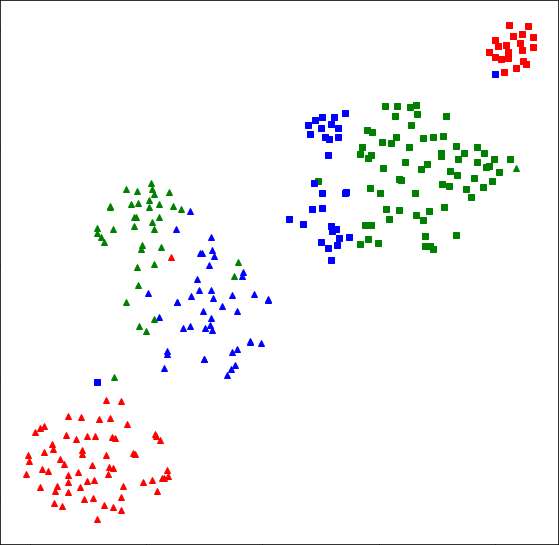
\includegraphics[width=10cm]{img/common_projection}
  \end{center}
  \caption{Basic projection of one knowledge component in Umíme česky}
  \label{fig:commonprojection}
\end{figure}

Figure \ref{fig:commonprojection} shows how common projection looks
like. This particular projection shows 273 items of single concept from
system. Each item is represented as one dot in the image and its
proximity to others represents how similar they are.

\subsection{Visible Properties of
projection}\label{visible-properties-of-projection}

% Visible Properties of projection

%% Similar words near each other

\begin{figure}
  \begin{center}
    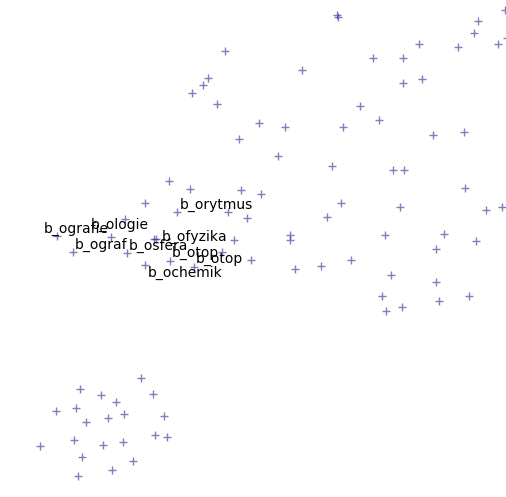
\includegraphics[width=10cm]{img/similar_words}
  \end{center}
  \caption{Similar words close to each other}
  \label{similarwords}
\end{figure}

we want to use results of calculated similarity and projections for
managing item pool. That puts some constrains on how ideal results look
like.

We want similar items to end as close to each other as possible. When
using performance as data source this is especially items using same
skill are projected near each other. E.g. figure \ref{similarwords}
shows projection of questions about Czech language with highlighted a
few similar words. This group consists of words witch are based on
single word with added suffix.

%% Regularities

%% This causes similar words to end-up far away one from another

After looking at image you can notice some regularities.

\subsubsection{Computation of item
similarity}\label{computation-of-item-similarity}

%% How is projection (similarity) computed

To better understand how was this image created we have to understand
how it is computed. We will describe it following section. This is
default work-flow we used in most cases. Whenever we don't specify
otherwise all projections were produced using this work-flow.

%%% Performance matrix

First step we have to do is converting raw logged information about
user answers to performance matrix. This matrix consist of entries for
each user-item pair. Columns of the matrix are items in educational
system and each row of the matrix contains data about single user's
performance. In most cases we used correctness of first users answer
to specific item as his performance. This means value 1.0 in case of
correct answer and 0.0 for incorrect. Another possible choice is to
incorporate user solving time into this value. TODO possible choices
are described in article {[}{]} Performance matrix is relatively
sparse as it is not common for users to solve all the items in the
system.

I tried using both first users answer and last in performance matrix.
However there is no visible difference in resulting projection (same
clusters are formed). This is clear when we compare first and last
answers of users. There is only 5% difference between them. So at least
with large number of items in system it doesn't really matter which one
is chosen.

%%% Similarity matrix

Next step is computing similarity matrix. Matrix $S$ is square
matrix where each position $S_{ij}$ denotes similarity of items
$i$ and $j$. In our case similarity is computed as correlation of
two columns $i$ and $j$ in performance matrix. This means we look
only at users who solved both items $i$ and $j$ and compute
Pearson correlation coefficient of their performance.

%%% PCA, (TSNE)

The last (optional) step is producing 2D projection. This can be
achieved by using many techniques for computing low dimensional
projections.

%%%% PCA over TSNE

We choose to use Principal component analysis (PCA) and there is several
reasons for doing so. Result of PCA is deterministic. It produces same
result for same input. This is not true for TSNA which is technique
using machine learning and gradient descent for finding some local
extreme. Stable results are more suitable for understanding data as
there is one less variation to results caused by algorithm. It is easier
to compare results when altering metrics used fro computing item
similarities.

First two principal components of PCA are then used for 2D
visualizations.

%%% Why this work-flow, performance data (not item statement)

We choose this specific work-flow as we think it is utilizing data about
items which hold most information about their similarity. As other
possible choices are item statement and solutions provided by students
they do not hold as much information. Item statements in our particular
exercises consist only of few Czech words. Also student solution is only
choice from two provided options. Item statement and solutions can be
used more effectively in other contexts like programming, mathematics,
physics, or chemistry.

This choice of work-flow is also relatively simple and easy to
understand. It consist of few steps which can be studied separately and
interchanged.

\subsection{Level regularity}\label{level-regularity}

% Level regularity %% Description of problem, 3 clusters based on 3
levels of questions difficulty

When you look back at figure \ref{fig:commonprojection} you can see that
there are three colors of items. Most TODOknowledge components in system
Umíme česky are spitted into multiple levels of difficulty. For this
particular knowledge component there are three difficulty levels. First
level is shown with red, second with green and third blue. This shows
visible pattern in our data - each color (level) forms a distinct
cluster. In following section we will try to explain factors that can
affect resulting projections produced from real-world data.

As we mentioned before, only data about user performance (correctness of
answers) are used when composing projections. And there is not a direct
reason for this clusters of same levels to form as no information about
belonging to particular level is presented to the algorithm.

%%% cause? how users tend to solve them

Levels are not solved uniformly. It is not common for user to sole all
three levels. Less experienced users tend to solve only first or first
two levels. However typically older users solve only higher levels. Main
cause for this is that system allows teachers to assign particular level
of concepts as homework. Students then usually solve only this single
level.

%%% why is this unsuitable

%%%% Example of similar words far away one from another

This phenomenon is not suitable for analysis of item similarity as it
can cause misleading results. One particular example is when similar
word are displayed far away form one another just because they belong to
different levels. This is visible for words ``bič'' and ``bičík'' in
problem set ``Vyjmenovaná slova B''.

\subsubsection{Sparseness of performance
matrix}\label{sparseness-of-performance-matrix}

%% question? can missing data affect result of similarity calculation

%%% Simulated data experiment

For purpose of determining this, we designed an experiment. writing
script that simulated answers provided by virtual students. Main problem
we wanted to recreate was missing data in performance matrix. Each
simulated user solved level and then with some probability continued to
another. So most users answered only to one level, some users to 2
levels and only few to all 3 levels. Levels were chosen at random as
users are not required to continue chronologically. Good enough as users
do not solve levels in order from easy to hard. There are also users who
solve only second or only highest difficulty level.

Results indicate that that structure of data can affect results only in
really special cases. But this is not our case. The only case where
projection is divided into clusters is when there is absolutely no
performance data between any question of groups.

\subsubsection{Users similarity
projection}\label{users-similarity-projection}

Insead we choose to analyse whether our data contains different groups
of users. We are changing how we are looking at data.Up until now we
used item-item similarity to calculate projection of items. Now we are
going to to be using user-user similarity.

It is worth mentioning we will work with larger matrices as this forced
us to do some optimalizations in code of our analysis. For example
similariy matrix of items usualy has size between $100\times 100$ and
$300\times 300$. As we are looking only on items from single knowledge
component. Hovewer user similarity matrix is square matrix with size
around $10 000\times 10 000$. This is also reason why current
recommender systems use item similarity instead of user similarity. CITE

First attempt on projecting users can be seen in figure ??.

% TODO users similarity

We say that user solved level when he anwered at least 30 questions
(which is 1/3 of questions for observed item set). Based on this we can
divide users into 8 groups. We added color to each group so we can
distinguish them in folowing plots easily.

\begin{center}
  \begin{tabular}{|c|c c c c c c c c|}
    \hline
    Group: none & only 1st level & only 2nd level & only 3rd level & both 1th and 2nd & both 2nd and 3rd & both 1nd and 3rd & all levels \\
    \hline
    Color: black & red & green & blue & yellow & cyan & magenta & light gray \\
    \hline
    Users count & 4984 & 4375 & 1285 & 1114 & 960 & 224 & 240 & 1025 \\
    \hline
    User & 35 & 31 & 9 & 8 & 7 & 2 & 2 & 7 \\
    \hline
  \end{tabular}
\end{center}

We can see that all formed custers of users contains in most cases users
from single user group when we divide them by levels they solved. This
brought us to more interesting discoveries. In general each level and
each item has some mean performace. This is shown in figure ??.
Horizontal axis contains items sorted by level and mean performance.
Vertical axis shows pwerformance of each item. Given item sets have mean
performance 94%, 86%, 71% for each level respectively.

After dividing users into 8 groups plot changes slightly. Some groups
like ``only 1st level'' (its colored red and contains users who solved
primarly first level and only few or none items from other levels) has
much lower performance on other levels. We can conclude that users who
tend to solve mostly first level arent as experienced as other users. On
other hand users in group ``both 2nd and 3rd'' (cyan) are performing
better than other users on all three levels.

At this point we have to return to simulation. We want to show that
grouos of users solving levelswith different performancecan cause
forming of clusters of items from same level.

Answers are simulated pretty mutch same as in previous simulated
experiments. We have 300 items divided into 3 levels. There is 3000
simulated users. Most of them solve levels with same skill but some 1/5
of users have smaller chance to solve second and third level. This is
visible on item performance polt similar to one from real data.

Only chnged variable was performance of some users for levels and this
resulted in visible clusters in projection (figure ??).

From otained information we can conclude that removing subnormal answers
of users (few answers to other levels when they solved primarly one
level) should remove clusters of levels.

But does it?!?

\subsection{Different performance
metrics}\label{different-performance-metrics}

% Different performance metrics

We applied 4 different metrics for computing similarity matrix to verify
that previous results aren't specific to single metric. Especially if it
is true that similarity of items differ based on correct answer.

%%% what different measures measure

Pearson and yule produce almost identical results - this confirms
previous research. This means plots produce same distinct clusters of
answers and total similarities. However Jaccard measurement differs in
this aspect. Similarity of items is not greater in one group of
questions (based on correct answer).

Different methods for computing similairty may measeure diferent aspects
of items. This can be seen when using Jaccard an Sokal metrics.
SImilarities provided by Jaccard metric differe greatly from other
metrics. Resulting projection still shows same clusters of level and
items are splited based on correct answer but information is kept in
another way than in correlation based metrics like Pearson.

On other hand Sokal is heavily depending on performance of items. Items
with higher performance are much more similar than items with lower
performance. This is causing packed cluster of first level (easy) and
spread out cluster of items from third level (harder).

%% Quantification of level clustering, split and compare with truth

\subsection{Answer regularity}\label{answer-regularity}

% Answer regularity %% Description of problem, items are divided into
clusters based correct answer (i/y) when there is no information about
this in data used for computing similarity

%%% TODO Outsider detection using similarity data

When exploring data, it may be useful to detect outsiders. It may be
useful for multiple reasons {[}TODO cite{]}. In our aprticular case we
declare item an outsider when it is not somilar to any other items in
problem set. seems like a logical path to take.

In particular this means item with low sum of similarities to other
items may be an outsider. This is where we encountered another
regularity in data.

%% Total similarity

Sum of similarities is sum of one column of simialrity matrix which we
produced in our workflow for computing projection.

\begin{figure}
  \begin{center}
    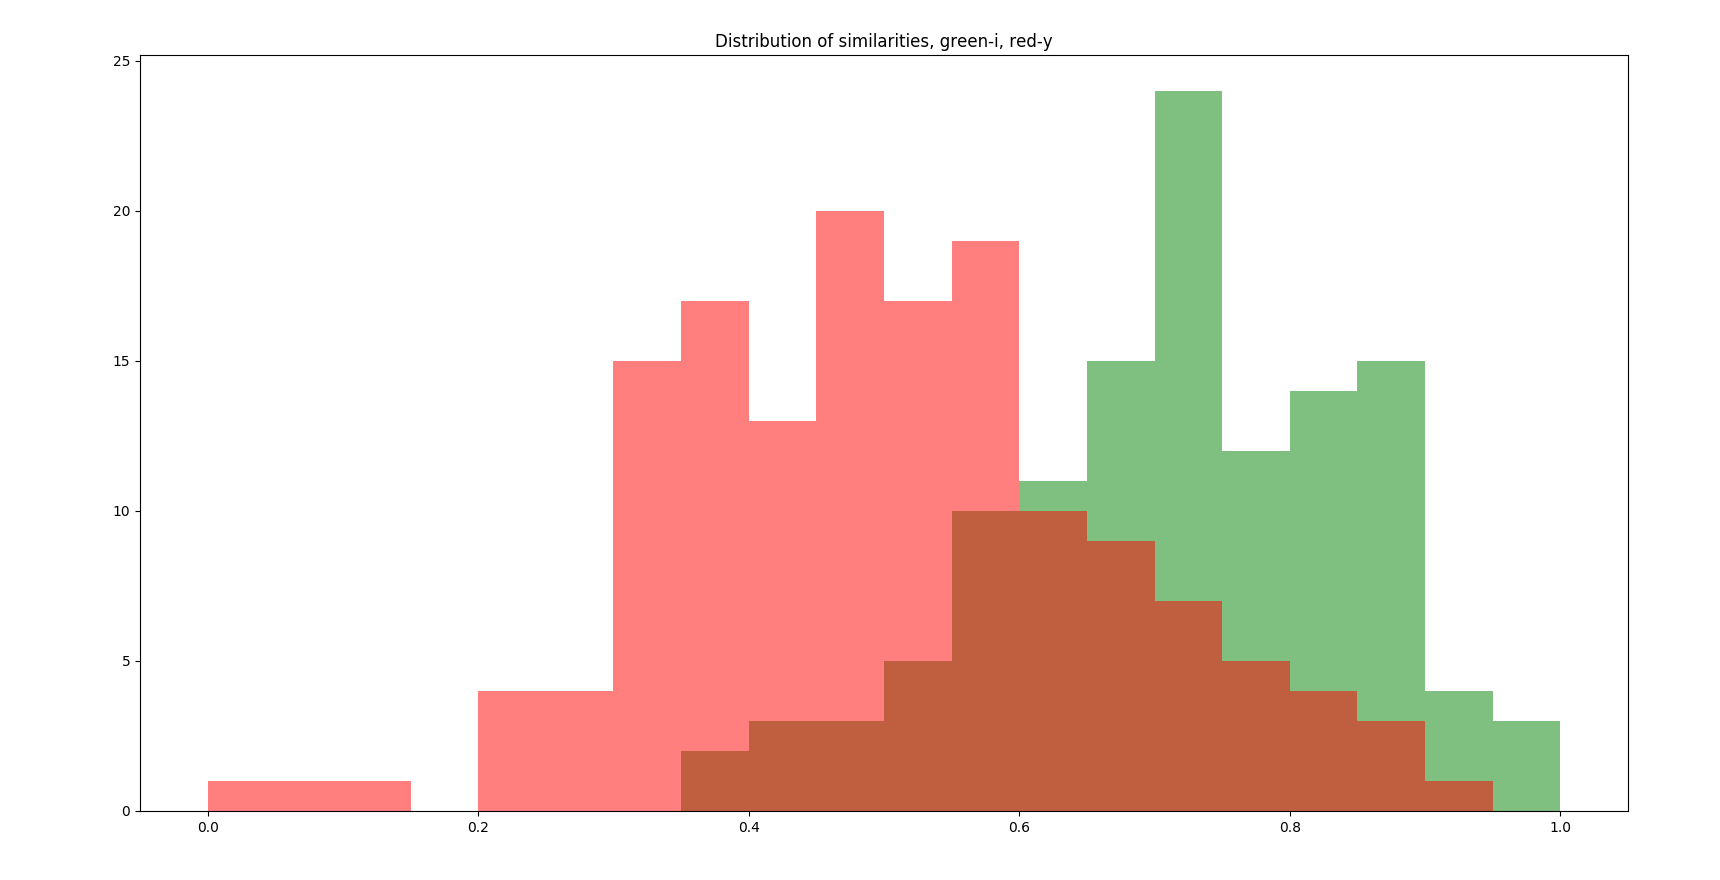
\includegraphics[width=10cm]{img/iy_histogram}
  \end{center}
  \caption{Histogram of similarities}
  \label{ref:iyhistogram}
\end{figure}

%%% total similarity histograms by answer

%%% quantification for different concepts

This is not specific to only one problem set (which was used in previous
images), almost all problem sets display similar pattern. However for
some its more distinct than for others. (Sets consisting of items with
many possible answers do not behave this way. But that is to be
expected.)

%% Users are choosing one answer by default when they do not know
answer

Our next experiment was simulation of users preferring one answer in
case they do not know what is the correct answer.

Answers are simulated for each user and question. There are no missing
values. Answer is correct whenever random value is higher than logistic
function of (users skill) - (difficulty of question). Half of questions
has one correct answer and other half another answer. We used this to
shift chance of answering correctly higher or lower (+0.1 for first
answer and -0.1 for second).

%\includegraphics{simulated_projection.png}
%\includegraphics{simulated_correlation_similarity_performance.png}

Colors represent answer of each item (chance shifted up or down). There
are formed visible clusters of same answers in result similar to
real-wold data. Using two uncorrelated skills cause clusters in
projection. (When using only single skill for all questions results does
not change and they are not required for this simulation.)

%%% it is usually answer on left, but there are exceptions koncovky
pridavnych mien je to Y (v pravo)

This is not specific to only one category (which was used in previous
images), many more categories display similar pattern. However for some
its more distinct than for others. For some distribution of similarities
is same for all answers (psani-nn-a-n, vyjmenovana-slova-po-p,..).

I picked few witch have very distinct answers and looked whether it is
answer on left or on right in user interface.

%%% % \textbar{} category \textbar{} answer with higher similarity
%%% \textbar{} position in UI \textbar{} % \textbar{}
%%% -------------------------------------- \textbar{}
%%% ----------------------------- \textbar{} -------------- \textbar{} %
%%% \textbar{} koncovky-podstatnych-jmen-muzsky-rod \textbar{} i \textbar{}
%%% left \textbar{} % \textbar{} koncovky-podstatnych-jmen-zensky-rodce
%%% \textbar{} i \textbar{} left \textbar{} % \textbar{}
%%% koncovky-podstatnych-jmen-stredni-rod \textbar{} i \textbar{} left
%%% \textbar{} % \textbar{} koncovky-pridavnych-jmen \textbar{} y
%%% \textbar{} right \textbar{} % \textbar{} psani-me-mne-ve-slove
%%% \textbar{} (m)ne \textbar{} left \textbar{} % \textbar{}
%%% me-mne-samostatne-zajmeno-ja \textbar{} (m)ne \textbar{} left \textbar{}
%%% % \textbar{} psani-be-bje \textbar{} (b)je \textbar{} left \textbar{}
%%% % \textbar{} vyjmenovana-slova-po-b \textbar{} i \textbar{} left
%%% \textbar{} % \textbar{} \ldots{} \textbar{} \ldots{} \textbar{}
%%% \ldots{} \textbar{}

%%% how to detect this in performance data? / what can we detect in
data?

%% Division of user answers 50-50, but not for correct answers

We observed before that whole data set uses both answers the same but
for single user this may not be true. There are even users who use only
one answer as seen in following performance matrix. There is a line with
all questions answered incorrectly for one answer and correctly for
another.

%\includegraphics{uneven_answers_perforamnce_perf_matrix.png}

We can filter this users out. Next three images show different levels of
filtering. First uses no filtering at all (uses all users). Second and
third image filter users by difference between performance on each
answer. (So if users has same performance on question with both answers
this value is 0.0 and when user uses only one of the answers (biggest
possible difference) value is 1.0). Second image shows value of 0.3
(performance on one answer is 30% higher than on the other one). And
third image uses value 6% which is median.

%\includegraphics{uneven_answers_perforamnce_none.png}
%\includegraphics{uneven_answers_perforamnce_0_3.png}
%\includegraphics{uneven_answers_perforamnce_half.png}

When we use only half of users which have uniform answers there are no
clusters of question with same answers. (Half of users because median is
used as filtering value.)

We can look at histogram of difference between answers. For most of the
users there is almost no difference but there are users with higher
difference in performance between answers.

%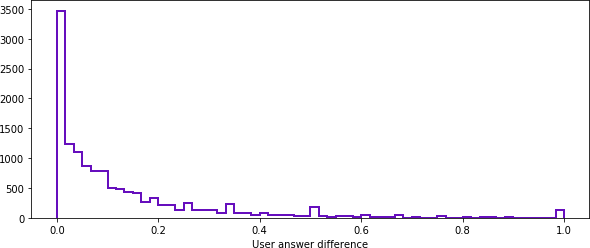
\includegraphics{uneven_answers_hist.png}

I look at difference between performance (amount of correctly answered
questions) instead of usage of each answer because it is performance
that affects calculated similarity of questions. However they should
correlate somewhat. Another reason is that it is closer to simulated
experiment so we can compare results directly.

When we simulated users we gave them all habit to use one answer more
commonly. But not all users have this habit in real-wold data. However
there is quite large amount of users who do.

This resolves first problem we encountered but does not explain other
regularities in data.

We succseeded in simualting data with clusters of same answers and
showing that this is case in our real data. Hovewer there is still one
more thing to explain - clusters of uqesrions with same levels.
Folloving same approach we can try to filter out users with large
difference in how successfuk they are with solving different levels.

Weused histogram of differences (variance of solved levels) to choose
some value for filtering of users. As more than half of users solves
only one level median of differences is 0.0. So we choose one value just
by looking at histogram. We can see in following figure that this dosnt
really matter as filtering users in this way does not help with
eliminating clustrs of same levels.

%% Levels of similarity

\subsection{Second level of
similarity}\label{second-level-of-similarity}

{[}Measuring Similarity of Educational Items Using Data on Learners'
Performance{]} suggests applying one additional level of correlation to
item similarity matrix. This means we are looking if items are behaving
similarly with respect to other items. First two images (top) show data
using only computed similarity of items. Second set of images shows same
questions after applying Pearson correlation to similarity matrix. Plots
on left show different possible answers (i/y) and plots on right
difficulty levels of questions.

Applying one additional level of correlation to item similarity matrix
was suggested {[}TODO{]}. This means we are looking whether items are
behaving similarly with respect to other items instead of similarity of
user performance directly.

We can study possible usage of this technique little further

One approach is take a step back, do not use any similarity at all and
compute projection directly from performance matrix. This is usually not
useful as performance matrix has large amount of missing values and PCA
works only with full matrices. However it is useful for exploring how
adding computation of similarity affects projections.

We used only users who solved all questions.

\subsection{User similarity}\label{user-similarity}

% User similarity

For explaining patterns of aquestions from same level we have to dig
deeper and understand different fpgroups of users. One particular way
how to acjive this is using owrkflow similar to previous. Althought
there will be one difference, we will be using similarity of users
instead of items. (item-item similarity matrix, user-user similarity
matrix). This also meqns that we have to transpose performance matrix -
so each column represents one user. Calculating correlarion between all
columns gives us user similarity matrix. There is no difference in
projection step, only used matrix is interexchnaged.

W pe ca.n try ploting this result direcly using PCA. Hovewer we would
notice that resulting image doesnt give us much information about users.
reason for this is that two principal components reflect some property
of data that we know about and dont wqnt to display. In particular users
solving only one group are somewhat special. Columns representing users
like this cannot be compared when they solved different levels - there
is missinf information about their correlarion. PCA chooses this
information with highest magnitude In presented figure this coresponds
to choosen components reflecting solving of first and third level.
(third principal domponent is corelates with solving of second level)

As users who solve only one level cause this behaviour. And they dont
give us information about similarity of items in different levels we
choose to exclude this users. After doing so we end up with projection
similar to figure xx.

There are two visible clusters of users. Futher analysis shows that
difference beween groups of users is caused by ?

\subsection{Another context}\label{another-context}

% Replicated in another context of math

%% (re)Usage in other concepts

\section{Conclusion}\label{conclusion}

% --------------------------- %
% Conclusion %
% --------------------------- %

We can conclude some recommendations. While trying to explain patterns
in our particular used data we run into multiple situatutions hwich can
repeat even when explaing some different data using similalr techniques.

Technique we used for calculating projections is quite common in area of
Adaptife learning and recommender systems. CITE.

Following section will summarize recommendations useful for explaining
results - it is useful to look at both item and user similarity - some
patterns in data can be results of habbits of users. - we are using
unsupervsed learning like techniques - we obtain some results but it is
hard to explain why they are like they are.. one possibility how to
explain results is using simulations - we explained one possible way of
simulating performance matrix - data fome from users so identifing
groups of users who behave same may be useful - we rhink most common
groups which can be vosibke in data coming from online tutoring system
are eager users and trolls - Main grohp of users tend to answer to
quesrions in some regullar patrern based on their knowledge while trolls
follow different pattern (for exampla use same answer on all questions)
- looking at total similarity of items - typicaly correlates with first
dimension of PCA - variance of performance entries of items


  \makeatletter\thesis@blocks@clear\makeatother
  \phantomsection %% Print the index and insert it into the
  \addcontentsline{toc}{chapter}{\indexname} %% table of contents.
  \printindex

\appendix %% Start the appendices.
\chapter{An appendix}
Here you can insert the appendices of your thesis.

\end{document}
